%% APEX — ASE 2026 Tools & Datasets Track
%% 4 pages max, ACM Proceedings Template, NOT double-blind.
%% Compile: latexmk -pdf main.tex   (needs texlive-publishers / acmart >= 1.90)
%% Or upload the whole docs/paper-ase2026/ folder to Overleaf, project type "ACM".
%%
%% Submission build uses [sigconf,review] (line numbers on). Camera-ready: drop "review".
\documentclass[sigconf,review,anonymous=false]{acmart}

%% --- draft conveniences: suppress the copyright strip / reference block while reviewing ---
\settopmatter{printacmref=false}
\setcopyright{none}
\renewcommand\footnotetextcopyrightpermission[1]{}
\pagestyle{plain}
%% ------------------------------------------------------------------------------------------

\usepackage{booktabs}
\usepackage{tikz}
\usetikzlibrary{positioning,arrows.meta,fit,backgrounds,calc}

%% Conference metadata (placeholder; the ACM TAPS pipeline will overwrite for camera-ready).
\acmConference[ASE 2026]{IEEE/ACM International Conference on Automated Software Engineering}{November 2026}{Location TBD}
\acmYear{2026}
\acmISBN{}
\acmDOI{}

\begin{document}

\title{APEX: A Self-Improving Harness for LLM Coding Agents Across the Software Lifecycle}
%% Alternate titles considered (pick one before submission):
%%  - APEX: A Phase-Gated, Self-Correcting Workbench for LLM-Based Software Development
%%  - APEX: Giving an LLM Coding Agent a Persistent, Self-Tuning Substrate

\author{Vicente Rivas Monferrer}
\affiliation{%
  \institution{VRAIN, Universitat Polit\`ecnica de Val\`encia}
  \city{Val\`encia}\country{Spain}}
\email{TODO@upv.es} %% <-- replace before submission

\author{Juan Miguel Alberola}
\affiliation{%
  \institution{VRAIN, Universitat Polit\`ecnica de Val\`encia}
  \city{Val\`encia}\country{Spain}}
\email{jalberola@dsic.upv.es} %% <-- verify

\author{V\'ictor S\'anchez-Anguix}
\affiliation{%
  \institution{VRAIN, Universitat Polit\`ecnica de Val\`encia}
  \city{Val\`encia}\country{Spain}}
\email{visanan1@upv.es} %% <-- verify

\author{Vicente Juli\'an}
\affiliation{%
  \institution{VRAIN, Universitat Polit\`ecnica de Val\`encia}
  \city{Val\`encia}\country{Spain}}
\email{vinglada@dsic.upv.es} %% <-- verify

\renewcommand{\shortauthors}{Rivas Monferrer et al.}

\begin{abstract}
LLM coding agents such as Claude Code now run multi-day, multi-project software
work, yet they degrade over long horizons: they lose context, forget which tools
exist, repeat errors made days ago in other projects, drift between development
phases, and declare phases ``done'' against mock data. We present \textbf{APEX}, a
harness that gives a coding agent a persistent, self-correcting cognitive
substrate. APEX layers entirely on top of an existing agent's extensibility
primitives---tool servers, lifecycle hooks, declarative skills, sub-agents---and
adds: (i) a phase-gated software lifecycle (14 phases, from a Socratic intake to
maintenance) whose transitions are guarded by deterministic-first checks; (ii) a
per-project temporal context database plus a cross-project hub that re-injects past
lessons at session start; and (iii) a self-improvement loop (an outcome-based
grader, an advisor sub-agent, a host-introspective ``doctor'', and a skill forge)
that proposes fixes to the harness itself. The artifact is open source, ships 620
passing tests, exposes 53 tool endpoints and 24 skills, and has been the working
harness for \(\approx\)20 real software and research projects. We describe the
design, walk through a session, and report what is and is not yet validated. A
five-minute screencast accompanies the paper.
\end{abstract}

\begin{CCSXML}
<ccs2012>
<concept><concept_id>10011007.10011074.10011099</concept_id><concept_desc>Software and its engineering~Software development methods</concept_desc><concept_significance>500</concept_significance></concept>
<concept><concept_id>10010147.10010178.10010179</concept_id><concept_desc>Computing methodologies~Intelligent agents</concept_desc><concept_significance>300</concept_significance></concept>
</ccs2012>
\end{CCSXML}
\ccsdesc[500]{Software and its engineering~Software development methods}
\ccsdesc[300]{Computing methodologies~Intelligent agents}

\keywords{LLM agents, agentic software engineering, developer harness, context
engineering, self-improving systems, Claude Code, Model Context Protocol}

\maketitle

%% =====================================================================
\section{Introduction}
%% =====================================================================
General-purpose LLM coding agents---Claude Code, Cursor's agent mode, OpenAI
Codex CLI, and open clones---are now used not as autocomplete but as the operator
of whole software tasks: they plan, edit files, run shells, call services, and
iterate over many turns~\cite{liu2026divecc}. As tasks lengthen from minutes to
days and span several repositories, a different failure mode dominates. It is not
that the model writes a bad line; it is that the \emph{harness around the model}
has no memory and no discipline. Concretely, in our own use of one such agent we
repeatedly observed: (a) \textbf{context amnesia}---a decision settled on Monday
re-litigated on Wednesday; (b) \textbf{forgotten capabilities}---bespoke tools and
skills that exist but are never invoked; (c) \textbf{cross-project error
recurrence}---the very mistake that broke project~A made again in project~B; (d)
\textbf{phase drift}---jumping to implementation before the spec or the threat
model exists; and (e) \textbf{premature ``done''}---marking an integration phase
complete with hard-coded mock data. Studies of multi-agent LLM systems report
production failure rates of 41--87\%, attributed predominantly to coordination
rather than to model capability~\cite{nechepurenko2026coord}; the single-agent,
long-horizon case is less measured but the symptoms above are familiar to any
practitioner.

Recent work names the response to this: \emph{harness
engineering}~\cite{zhou2026external}---building the runtime infrastructure
(memory stores, skills, protocols) that earlier systems hoped the model would
reconstruct internally. ``Dive into Claude Code''~\cite{liu2026divecc} documents
the four extensibility mechanisms a modern agent exposes---tool servers (MCP),
plugins, declarative skills, and lifecycle hooks---plus sub-agent delegation. The
self-evolving-agents survey~\cite{fang2025selfevolve} casts the ideal system as a
four-part loop (System Inputs, Agent System, Environment, Optimisers) and notes
that most deployed agents are statically configured. What is missing is a concrete
developer harness that (1) imposes a phase-gated lifecycle with
\emph{deterministic-first} gates, (2) carries a temporal context store that is
both per-project and cross-project, and (3) closes the loop by proposing changes
to \emph{itself}---all at once, on top of an unmodified commercial agent.

\textbf{This paper presents APEX}, an open-source harness that does exactly that.
Our contributions are: (1) the \emph{design} of a phase-gated agentic SDLC whose
phase transitions are blocked by a hook running deterministic checks before any
LLM judgement is consulted; (2) a \emph{context substrate}---a per-project SQLite
database with temporal facts, bidirectional error memory, and an FTS5 wiki, plus a
cross-project hub that re-injects past lessons at session start; (3) a
\emph{self-improvement loop}---an outcome-based grader, an advisor sub-agent under
a strict token/rate budget, a host-introspective ``doctor'', and a skill forge
that mines repeated patterns into proposed new skills; and (4) the \emph{artifact}
itself: 53 tool endpoints, 24 skills, 11 hooks, 620 passing tests, MIT-licensed,
archived on Zenodo, and used as the working harness for \(\approx\)20 real
projects over roughly two months. A five-minute screencast demonstrates a live
session.

%% =====================================================================
\section{Background: the agent harness}
%% =====================================================================
APEX is built on the extensibility surface that modern coding agents share; we
prototype on Claude Code~\cite{anthropic2025cc,liu2026divecc}, but the design uses
only generic primitives. \textbf{Tool servers} (the Model Context
Protocol~\cite{anthropic2024mcp}) let an agent call out to user-defined
functions over a typed interface. \textbf{Lifecycle hooks} are scripts the agent
invokes at fixed points---\textsf{SessionStart}, \textsf{UserPromptSubmit},
\textsf{PreToolUse}, \textsf{PostToolUse}---and a \textsf{PreToolUse} hook can
\emph{block} the call it intercepts. \textbf{Skills} are Markdown files with YAML
front-matter (a name and a trigger description) that the agent loads on demand,
turning a procedure into a first-class, model-selectable capability.
\textbf{Sub-agents} are scoped child sessions with their own tool whitelist and
model, dispatched for a bounded task. APEX uses all four: an MCP server for the
context store and lifecycle operations, hooks for the gates and for context
injection, skills for the development procedures, and sub-agents for the advisor
and the per-phase ``virtual office'' roles. No model weights, no fork of the agent,
no API keys are required to run the harness; the agent's own subscription is the
only LLM.

%% =====================================================================
\section{APEX architecture}
%% =====================================================================
Figure~\ref{fig:arch} shows the layers. We describe each in turn.

\begin{figure}[t]
  \centering
  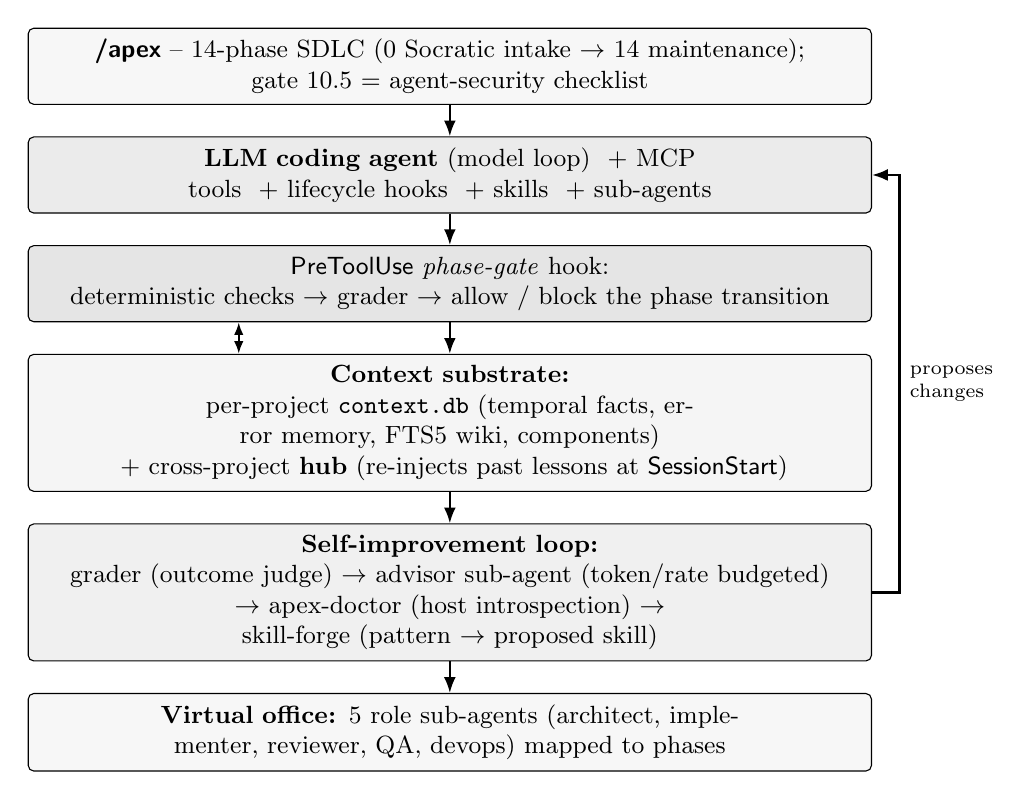
\begin{tikzpicture}[
      font=\small,
      box/.style={draw, rounded corners=2pt, align=center, inner sep=4pt,
                  minimum height=8mm, text width=.86\columnwidth},
      ar/.style={-{Latex[length=2mm]}, thick},
      node distance=4mm and 0mm
    ]
    \node[box, fill=black!3] (cmd)
      {\textbf{\textsf{/apex}} -- 14-phase SDLC (0 Socratic intake $\to$ 14 maintenance);\\ gate~10.5 = agent-security checklist};
    \node[box, fill=black!8, below=of cmd] (agent)
      {\textbf{LLM coding agent} (model loop) \ +\ MCP tools \ +\ lifecycle hooks \ +\ skills \ +\ sub-agents};
    \node[box, fill=black!10, below=of agent] (gate)
      {\textsf{PreToolUse} \emph{phase-gate} hook:\\ deterministic checks $\to$ grader $\to$ allow / block the phase transition};
    \node[box, fill=black!4, below=of gate] (ctx)
      {\textbf{Context substrate:}\\ per-project \texttt{context.db} (temporal facts, error memory, FTS5 wiki, components)\\ \ +\ cross-project \textbf{hub} (re-injects past lessons at \textsf{SessionStart})};
    \node[box, fill=black!6, below=of ctx] (loop)
      {\textbf{Self-improvement loop:}\\ grader (outcome judge) $\to$ advisor sub-agent (token/rate budgeted)\\ $\to$ apex-doctor (host introspection) $\to$ skill-forge (pattern $\to$ proposed skill)};
    \node[box, fill=black!3, below=of loop] (office)
      {\textbf{Virtual office:} 5 role sub-agents (architect, implementer, reviewer, QA, devops) mapped to phases};
    \draw[ar] (cmd) -- (agent);
    \draw[ar] (agent) -- (gate);
    \draw[ar] (gate) -- (ctx);
    \draw[ar] (ctx) -- (loop);
    \draw[ar] (loop) -- (office);
    %% feedback arrow routed in the right-hand margin (outside the boxes)
    \draw[ar] (loop.east) -- ++(3.5mm,0) |- node[pos=.25, right, font=\scriptsize, align=left] {proposes\\changes} (agent.east);
    %% the gate reads/writes the context substrate (short two-way hint)
    \draw[{Latex[length=1.6mm]}-{Latex[length=1.6mm]}, thick] ($(gate.south west)!0.5!(gate.south)$) -- ($(ctx.north west)!0.5!(ctx.north)$);
  \end{tikzpicture}
  \caption{APEX layers on the agent's own extensibility primitives. A
  \textsf{PreToolUse} hook gates phase transitions; the context substrate is both
  per-project and cross-project; a self-improvement loop proposes changes back to
  the harness.}
  \Description{A vertical layered diagram. Top: the /apex 14-phase software
  lifecycle command with a security gate at 10.5. Below it: the LLM coding agent
  loop with MCP tools, hooks, skills and sub-agents. Below that: a PreToolUse
  phase-gate hook that runs deterministic checks then the grader before allowing or
  blocking a phase transition; it reads and writes a per-project context database
  on the left and a cross-project hub on the right. Beneath: a self-improvement
  loop chaining grader, advisor sub-agent, apex-doctor and skill-forge. Bottom: a
  virtual office of five role sub-agents mapped to phases.}
  \label{fig:arch}
\end{figure}

\subsection{A phase-gated software lifecycle}
The \textsf{/apex} command runs a 14-phase lifecycle: phase~0 is a Socratic intake
that decides whether the idea is well-formed enough to skip the interview;
phases~1--3 cover problem framing, design (with a competitor scan and a validated
\textsf{DESIGN.md} carrying real tokens), and a checkpointed spec; phase~4
enumerates edge cases \emph{before} code; phases~5--7 are TDD implementation;
phase~8 integration review; phase~9 QA with a coverage floor; phase~10 a security
audit; \textbf{gate~10.5} maps an eight-layer agent-security checklist to the work
and \emph{blocks phase~11 unless every layer passes}; phases~11--14 are deploy,
launch, scale, and maintenance. The command file also encodes eleven concrete
``do not repeat'' errors drawn from past projects.

The discipline is enforced, not advisory. A \textsf{PreToolUse} hook intercepts the
\textsf{apex\_set\_phase} tool. It first runs \emph{deterministic} checks---is git
initialised and are there commits? do the tests pass? is the OS what the stack
assumed? are there emoji in user-facing strings? is the required schema present?
do declared integration points resolve to real code rather than mocks?---and only
if those pass does it consult the outcome-based grader (\S\ref{sec:loop}). If
either says ``block'', the transition is refused with an actionable message. This
``deterministic-first'' ordering is deliberate: cheap, reproducible checks gate the
common failures; the LLM judge is reserved for what genuinely needs judgement.

\subsection{The context substrate}
Each project gets a \texttt{.apex/context.db} (SQLite, 25 tables, FTS5). It stores
\textbf{temporal facts}---decisions and components carry \texttt{valid\_from} /
\texttt{invalid\_from} timestamps, so superseded choices are retained but marked
stale rather than deleted (a Graphiti-style bi-temporal model); \textbf{a
bidirectional error memory}---each recorded error has a \texttt{recurrence\_count}
and links to the decision that should prevent it, so a repeat increments rather than
duplicates; \textbf{a wiki}---Markdown pages with front-matter and wiki-links,
full-text indexed; and \textbf{progressive disclosure}---the same context is
retrievable at three sizes (compact \(\approx\)200 tokens, timeline
\(\approx\)800, full \(\approx\)2000) so a session pays only for the depth it
needs. Retrieval is hybrid (BM25 over FTS5 plus keyword overlap).

A second database, the \textbf{hub}, aggregates across all APEX projects on the
machine. Its job is anti-amnesia at the \emph{ecosystem} level: a
\textsf{SessionStart} hook reads the hub and injects, at the top of every new
session in any APEX project, the critical errors recorded \emph{elsewhere}---so the
SwiftUI-on-Linux mistake made in one project becomes a guardrail in the next.

\subsection{The self-improvement loop}
\label{sec:loop}
Four components let the harness critique and patch itself.
\textbf{The grader} is an outcome-based judge: given a claimed accomplishment and
the project state, it runs deterministic checks (git status, test results, OS
assumptions, emoji, presence of Pydantic models / Playwright E2E, etc.) and, when
enabled, an LLM judge; it emits a verdict with a \texttt{should\_block} flag that
the phase-gate hook honours.
\textbf{The advisor} is an Opus sub-agent invoked behind a strict budget---it sees a
bundle capped at \(\approx\)2500 tokens, will not run unless at least eight tool
calls have elapsed since its last review, and a circuit breaker disables it above
three calls per minute---and returns short ``advice cards'' of four kinds
(forgotten-tool, phase-drift, recommend-skill-handoff, grader-overdue) that a
\textsf{UserPromptSubmit} hook surfaces to the operator.
\textbf{apex-doctor} runs three analysers over the context store---clusters of
errors with high recurrence or severity, grader-block patterns recurring across
phases, and stale hand-off files---and writes idempotent, deduplicated proposals;
it is triggered by \emph{intent} (a wrap-up phrase, or a session older than a
threshold), not by a cron.
\textbf{The skill forge} watches the tool-call log and the grader history; when it
sees the same blocking issue across \(\geq\)3 phases, a 3-tool sub-sequence
repeated \(\geq\)5 times, or a decision recurring across \(\geq\)2 projects, it
drafts a candidate \textsf{SKILL.md} into a proposals directory for the operator to
approve or reject (rejections are remembered). It can also ingest community skills
from public repositories, validating front-matter and scanning for leaked secrets
before proposing.
Finally, \textbf{reasoning traces}---short, categorised records of why the agent
did what it did at key gates---are logged per phase and exportable in ShareGPT
format, both as an audit trail and as future fine-tuning fuel.

\subsection{The virtual office}
Five role sub-agents---architect, implementer, reviewer, QA, devops---are installed
as native sub-agents with their own tool whitelists and APEX-aligned system prompts
(no emoji; Spanish prose for this user; consult prior decisions before proposing a
stack; never ship mock data). A phase\(\to\)role map recommends, e.g., the
implementer for phases~5--7 and the reviewer for phase~8; the orchestrator
dispatches the role via the agent's own \textsf{Task} mechanism. Because everything
runs under the operator's subscription, the office costs no API spend.

%% =====================================================================
\section{Using APEX}
%% =====================================================================
\textbf{Install.} Clone \texttt{apex-harness}, register the MCP server and the
hooks with the agent (a one-line config), and install the skills and role
sub-agents. \textbf{Run.} In a project directory, invoke \textsf{/apex}. On a new
idea the agent runs the Socratic round, then proposes an architecture and a
checkpointed spec; phase~4 forces an edge-case list; phases~5--7 implement
test-first, one vertical slice at a time, with git initialised at the very first
sub-step; phase~8 reviews the integration; phase~9 enforces the coverage floor and
runs Playwright E2E against the \emph{real} backend; phase~10 plus gate~10.5 do the
security pass and block deployment until clean; phases~11--14 ship and maintain it.
Throughout, every decision, error, and component is written to \texttt{context.db}
and mirrored to the hub; the advisor periodically nudges; \textsf{apex\_get\_context}
re-grounds the agent at any point at the cheapest sufficient depth. On an
\emph{existing} codebase, a reverse-engineering path scans the repo and back-fills
the substrate before the lifecycle resumes. The accompanying screencast shows a
session end to end: \textsf{/apex} starting, the phase-gate refusing a premature
transition, an advisor card firing, the grader verdict, and the hub injecting a
cross-project lesson.

%% =====================================================================
\section{Evidence of utility}
%% =====================================================================
APEX is not yet the subject of a controlled study; what we can report is the
following. The artifact ships \textbf{620 passing tests} covering the context
schema and retrieval, the grader and goal loop, the hand-off and token-budget
machinery, the doctor's analysers, the skill forge's detectors, the role registry,
and the prototype scaffolder. It has been the \textbf{working harness for
\(\approx\)20 real software and research projects} over roughly two months---web
applications, multi-agent systems, several university final-year projects and their
tooling, research-workflow tools, and APEX's own development (it is built with
itself). Across those projects the substrate has accumulated \textbf{322 recorded
decisions, 184 recorded errors} (with recurrence tracking and links to preventive
decisions), \textbf{279 components, and 160 wiki pages}, all aggregated in the
cross-project hub; the \textsf{SessionStart} injector currently re-surfaces five
\texttt{critical} cross-project lessons in every new session---among them, from one
project, ``propose a platform-dependent stack only after checking the OS'', ``never
use emoji as UI icons'', ``do not mark an integration phase complete against mock
data'', and ``initialise git as the first sub-step of implementation'', and from
another, ``data detected by an upstream agent must flow explicitly through the
shared context, not be re-derived downstream''. These were real mistakes; they are
now harness-enforced guardrails.

We are explicit about what is \emph{not} validated. The self-improvement loop
(grader, advisor, doctor, skill forge) is implemented and unit-tested but has only
just begun to be exercised in the field: the production databases hold a single
grader verdict, three doctor proposals, and one reasoning trace at the time of
writing. We therefore claim a working, self-instrumenting harness with substantial
field use of its memory layer---not measured improvement from its optimiser layer.
Quantifying that is the obvious next step.

%% =====================================================================
\section{Related work}
%% =====================================================================
\textbf{Harness engineering and externalization.} Zhou et
al.~\cite{zhou2026external} survey the shift ``from weights to context to harness''
and identify \emph{self-evolving harnesses} and \emph{shared infrastructure} as
open directions; APEX is a concrete instance of the former with the latter built in
(the hub). ``Dive into Claude Code''~\cite{liu2026divecc} documents the very
substrate APEX builds on (MCP, plugins, skills, hooks, sub-agents, layered
compaction) and lists open design questions; we answer one of them with a
working layer.
\textbf{Self-evolving agents.} Fang et al.'s survey~\cite{fang2025selfevolve}
frames the four-part loop in which APEX's grader/advisor/doctor/skill-forge are
\emph{Optimisers} acting on the \emph{Agent System}. SEVerA~\cite{banerjee2026severa}
constrains self-evolving agents with first-order-logic output contracts and formal
verification---a heavyweight alternative to APEX's pragmatic, SQL-predicate phase
gates; the two are complementary (one could verify a phase gate's predicate).
\textbf{Coordination as a layer.} Nechepurenko and
Shuvalov~\cite{nechepurenko2026coord} argue coordination should be a separate,
independently measured architectural layer in multi-agent systems; APEX applies the
same separation to a single agent---phase gating and role mapping are the
coordination layer, distinct from the agent's capability.
\textbf{Autonomous-agent frameworks.} Early autonomous loops (AutoGPT,
BabyAGI~\cite{autogpt2023,babyagi2023}) and orchestration libraries
(LangGraph~\cite{langgraph2024}, AutoGen~\cite{wu2023autogen}) provide the loop and
the plumbing but not a phase-gated SDLC, a temporal cross-project memory, or a
self-tuning step; APEX is closer to a methodology made executable than to a library.
To our knowledge no existing system combines deterministic-first \textsf{PreToolUse}
phase gates, a self-tuning improvement loop, and a cross-project persistent memory
hub in one developer harness.

%% =====================================================================
\section{Limitations and availability}
%% =====================================================================
\textbf{Limitations.} (1) Running the lifecycle end to end requires a commercial
coding agent (we prototype on Claude Code) and its paid subscription; the artifact
itself---the MCP server, hooks, skills, and the 620-test suite---is fully
inspectable and the tests run standalone, but a reviewer cannot reproduce a full
agentic session without that platform. (2) Evaluation is single-user so far; a
multi-user study is needed and planned. (3) The substrate is local-first SQLite;
team synchronisation beyond the file-based hub is future work. (4) Several skills
encode this user's conventions (Spanish prose, anti-emoji); they are configuration,
not core, but a reviewer should know.
\textbf{Availability.} Source: \url{https://github.com/vjrivmon/apex-harness}
(MIT). Archived snapshot with DOI: \url{https://doi.org/10.5281/zenodo.XXXXXXX}
(to be minted). Screencast (\(\leq\)5\,min, voiced): \url{https://youtu.be/XXXXXXXXXXX}.
Reproducing the test suite: \texttt{PYTHONPATH=lib .venv/bin/pytest tests/}.

\begin{acks}
This work was supported by VRAIN, Universitat Polit\`ecnica de Val\`encia.
%% Add grant numbers / projects here before submission.
\end{acks}

\bibliographystyle{ACM-Reference-Format}
\bibliography{references}

\end{document}
